\documentclass[a4paper,12pt]{article} % тип документа

% Поля страниц
\usepackage[left=2.5cm,right=2.5cm, top=2cm,bottom=2cm,bindingoffset=0cm]{geometry}

%Пакет дял таблиц   
\usepackage{multirow} 

%Отступ после заголовка    
\usepackage{indentfirst}


% Рисунки
\usepackage{subcaption,floatrow,graphicx,calc}
\usepackage{wrapfig}

% Создаёем новый разделитель
\DeclareFloatSeparators{mysep}{\hspace{1cm}}

% Ссылки?
\usepackage{hyperref}
\usepackage[rgb]{xcolor}
\hypersetup{				% Гиперссылки
	colorlinks=true,       	% false: ссылки в рамках
	urlcolor=blue          % на URL
}


%  Русский язык
\usepackage[T2A]{fontenc}			% кодировка
\usepackage[utf8]{inputenc}			% кодировка исходного текста
\usepackage[english,russian]{babel}	% локализация и переносы


% Математика
\usepackage{amsmath,amsfonts,amssymb,amsthm,mathtools, mathrsfs, wasysym}


\begin{document}
	\begin{center}
		\footnotesize{ФЕДЕРАЛЬНОЕ ГОСУДАРСТВЕННОЕ АВТОНОМНОЕ ОБРАЗОВАТЕЛЬНОЕ 			УЧРЕЖДЕНИЕ ВЫСШЕГО ОБРАЗОВАНИЯ}\\
		\footnotesize{МОСКОВСКИЙ ФИЗИКО-ТЕХНИЧЕСКИЙ ИНСТИТУТ\\(НАЦИОНАЛЬНЫЙ 			ИССЛЕДОВАТЕЛЬСКИЙ УНИВЕРСИТЕТ)}\\
		\footnotesize{ФАКУЛЬТЕТ ОБЩЕЙ И ПРИКЛАДНОЙ ФИЗИКИ\\}
		\hfill \break
		\hfill\break
		\hfill\break
		\hfill \break
		\hfill \break
		\hfill \break
		\hfill \break
		\hfill \break
		\hfill \break
		\hfill \break
		\hfill \break
		\hfill \break
		\hfill \break
		\hfill \break
		\large{Лабораторная работа № 6.10.4 \\\textbf{Магнитные моменты легких ядер\\установка №4}}\\
		\hfill \break
		\hfill \break
		\hfill \break
		\begin{flushright}
			Серебренников Даниил\\
			Группа Б02-826м
		\end{flushright}
		\hfill \break
		\hfill \break
		\hfill \break
		\hfill \break
		\hfill \break
		\hfill \break
		\hfill \break
		\hfill \break
		\hfill \break
		\hfill \break
		\hfill \break
	\end{center}
	\begin{center}
		Долгопрудный, 2021 г.
	\end{center}
	\thispagestyle{empty}
	\newpage
	\textbf{Цель работы:} вычислить магнитные моменты протона, дейтрона и ядра фтора на основе измерения их $g$-факторов методом ядерного магнитного резонанса (ЯМР).
	
	\section{Основные формулы}
	Фактор Ланде:
	\begin{equation*}
		\label{eq:g}
		\tag{$\star$}
		g_\text{я} = \frac{hf_0}{\mu_\text{я}B_0}.
	\end{equation*}
	Магнитный момент ядра:
	\begin{equation*}
		\label{eq:mu}
		\tag{$\star\star$}
		\mu = g_\text{я}\mu_\text{я}I.
	\end{equation*}
	Ядерный магнетон:
	\begin{equation*}
		\mu_{\text{я}} = \frac{e\hbar}{2m_pc} \approx 5,05\cdot10^{-27} \text{Дж}\cdot\text{Тл}^{-1}.
	\end{equation*}
	\section{Экспериментальная установка}
	\thisfloatsetup{floatrowsep=mysep}	
	\begin{figure}[h!]
		\begin{floatrow}
			\ffigbox[\FBwidth]{\caption{Схема экспериментальной установки.}\label{fig:ust}}
			{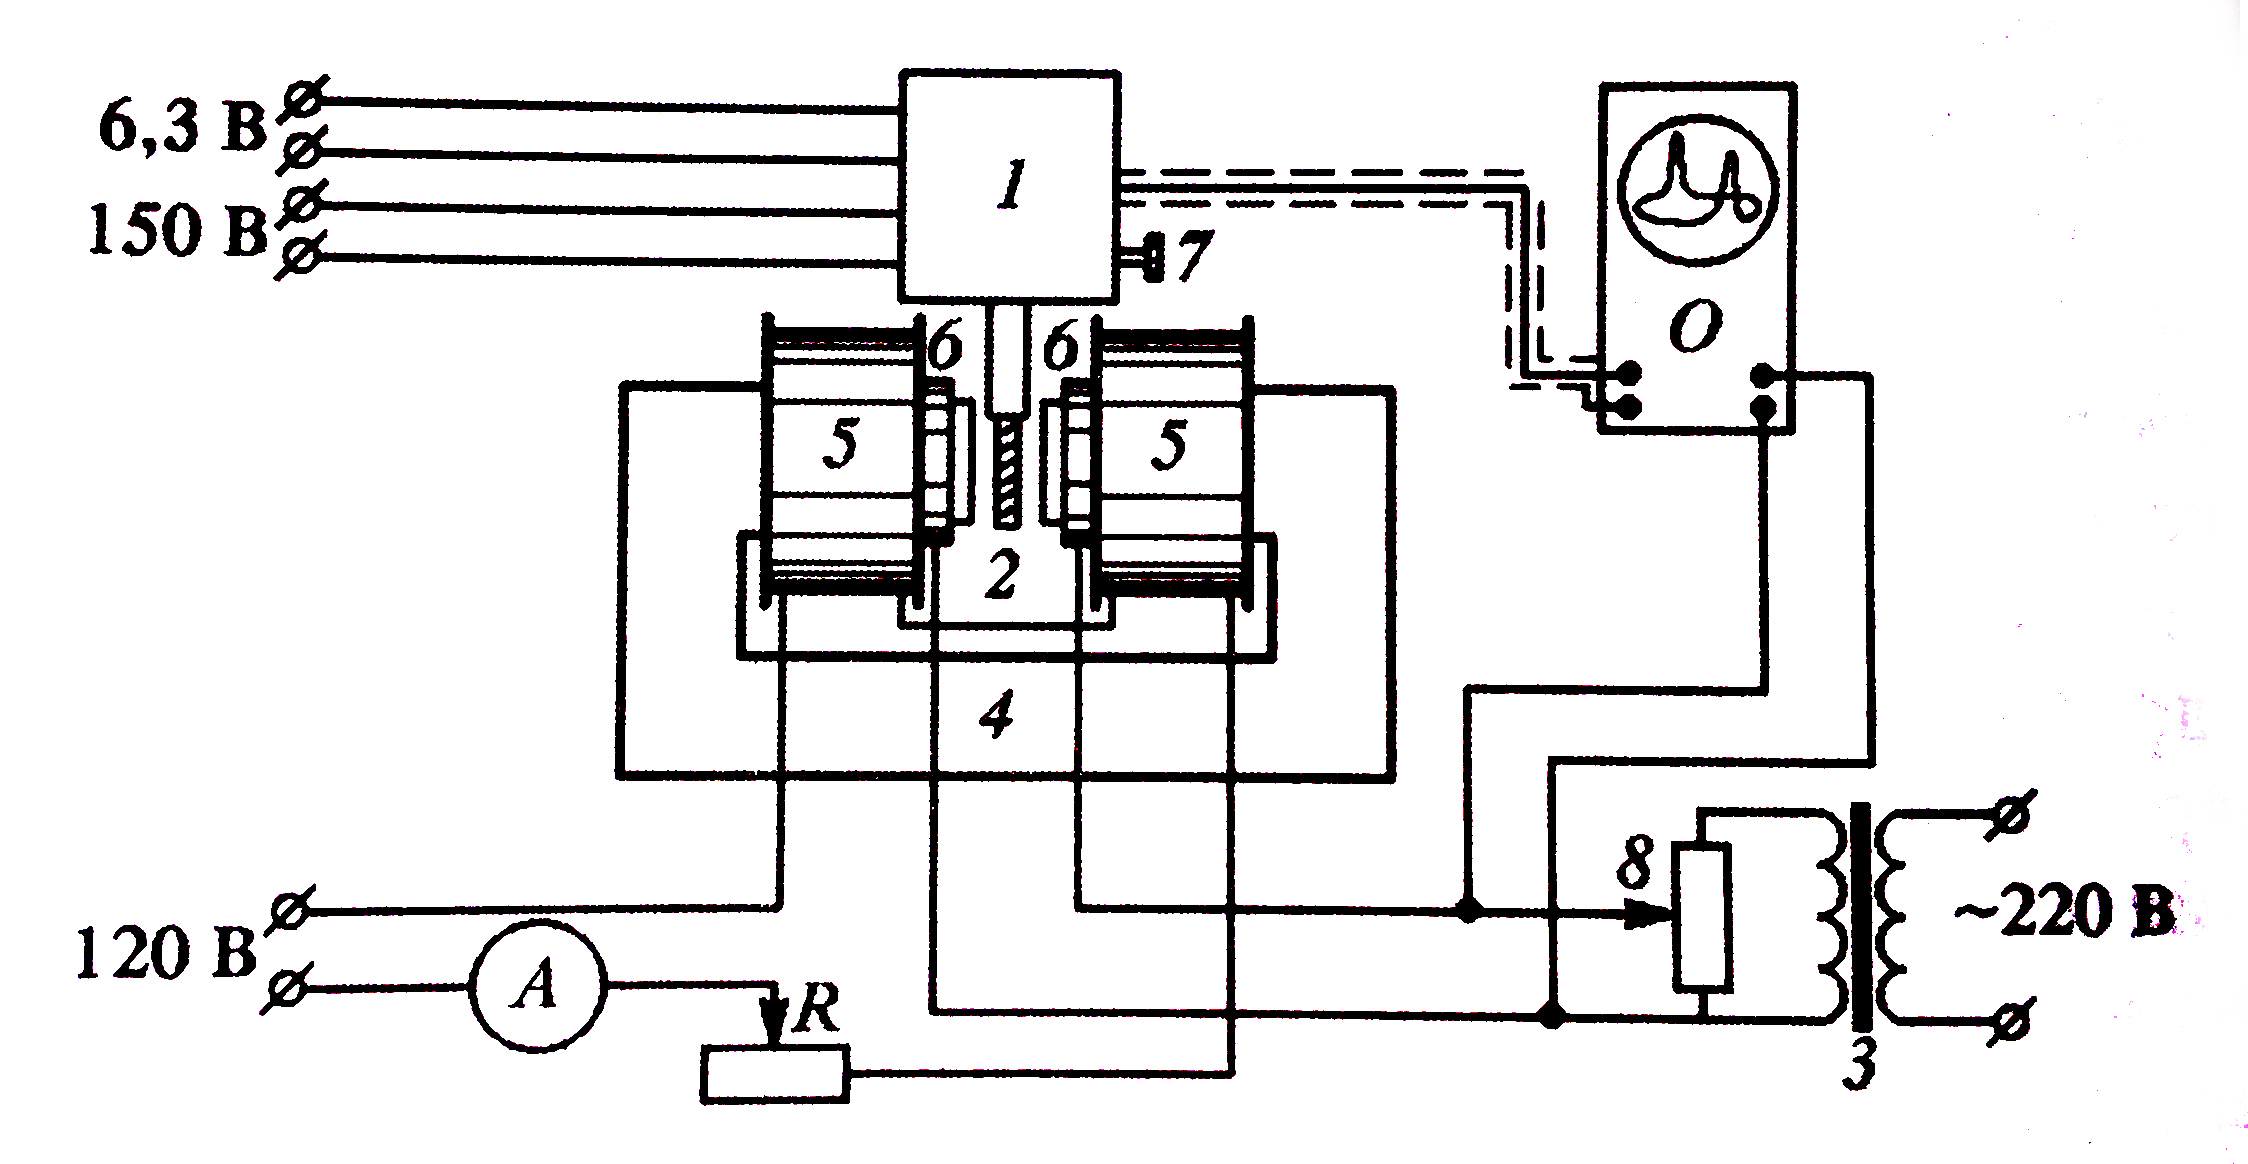
\includegraphics[scale=0.2]{ustanovka}}    
		\end{floatrow}
	\end{figure}
	\par 1. Генератор
	\par 2. Исслудуемый образец
	\par 3. Трансформатор
	\par 4. Электромагнит
	\par 5. Катушки, питаемые постоянным током, создающее основное магнитное поле
	\par 6. Моделирующие катушки, возбуждающие дополнительное поле
	\par 7. Лимб, меняющий емкость генератора, а следовательно, и частоту генератора
	\par 8. Потенциометр, регулирующий напряжение на катушках.

	\newpage
	\section{Экспериментальные данные}
	\begin{enumerate}
		\item
			$\sigma_{f_0} = 0,001$ Мгц;
		\item
			$\sigma_I = 0,01$ А;
		\item
			$\sigma_{B_1}  = 0,01$ мТл;
		\item
			$\sigma_{B_2} = 1$ мТл.
	\end{enumerate}
	
	\floatsetup[table]{capposition=top}	
	\begin{table}[H]
		\caption{Результаты измерений.}
		\label{table:exp1}
		\begin{tabular}{|c|c|c|c|c|c|c|c|c|}
			\hline
			\multirow{2}{*}{} & \multicolumn{4}{c|}{+}                        & \multicolumn{4}{c|}{-}                        \\ \cline{2-9} 
			& $f_0$, МГц & $I$, А & $B_1$, мТл & $B_2$, мТл & $f_0$, МГц & $I$, А & $B_1$, мТл & $B_2$, мТл \\ \hline
			Вода              & 9,853      & 0,33   & 231,43     & 231        & 9,867      & 0,33   & 231,75     & 231        \\ \hline
			Резина            & 9,160      & 0,31   & 215,14     & 214        & 9,173      & 0,31   & 215,44     & 215        \\ \hline
			Тефлон            & 10,155     & 0,38   & 238,53     & 252        & 10,162     & 0,38   & 238,67     & 252        \\ \hline
		\end{tabular}
	\end{table}
	
	\section{Обработка результатов}
		\begin{enumerate}
			\item
				Вода (ядро водорода):
				\begin{itemize}
					\item
						$g_\text{я} = 5,60 \pm 0,02$;
					\item
						$\mu = (2.80 \pm 0,01) \mu_\text{я}$.
				\end{itemize}
			\item
				Резина (ядро водорода):
				\begin{itemize}
					\item
						$g_\text{я} = 5,62 \pm 0,03$;
					\item
						$\mu = (2,81 \pm 0,15)\mu_\text{я}$.
				\end{itemize}
			\item
				Тефлон (ядро фтора):
				\begin{itemize}
					\item
						$g_\text{я} = 5,29 \pm 0,02$;
					\item
						$\mu = (2,65 \pm 0,01)\mu_{\text{я}}$.
				\end{itemize}
		\end{enumerate}
	
	\section{Обсуждение результатов и выводы}
		Методом ЯМР вычислены значения магнитных моментов ядер воды, резины и тефлона, то есть пртона и ядра фтора. Табличные значения магнитных моментов в пределах ошибки совпадают с экспериментальными результатами.
		
		Отметим, что $g$-фактор протона я ядра фтора близки, так как спин ядра фтора есть 1/2 (а не 5/2). Это обусловлено тем, что у фтора уровень $2s_{1/2}$ заполняется раньше.
	
	
\end{document}